% Options for packages loaded elsewhere
\PassOptionsToPackage{unicode}{hyperref}
\PassOptionsToPackage{hyphens}{url}
\PassOptionsToPackage{dvipsnames,svgnames,x11names}{xcolor}
%
\documentclass[
]{scrartcl}

\usepackage{amsmath,amssymb}
\usepackage{iftex}
\ifPDFTeX
  \usepackage[T1]{fontenc}
  \usepackage[utf8]{inputenc}
  \usepackage{textcomp} % provide euro and other symbols
\else % if luatex or xetex
  \usepackage{unicode-math}
  \defaultfontfeatures{Scale=MatchLowercase}
  \defaultfontfeatures[\rmfamily]{Ligatures=TeX,Scale=1}
\fi
\usepackage{lmodern}
\ifPDFTeX\else  
    % xetex/luatex font selection
\fi
% Use upquote if available, for straight quotes in verbatim environments
\IfFileExists{upquote.sty}{\usepackage{upquote}}{}
\IfFileExists{microtype.sty}{% use microtype if available
  \usepackage[]{microtype}
  \UseMicrotypeSet[protrusion]{basicmath} % disable protrusion for tt fonts
}{}
\makeatletter
\@ifundefined{KOMAClassName}{% if non-KOMA class
  \IfFileExists{parskip.sty}{%
    \usepackage{parskip}
  }{% else
    \setlength{\parindent}{0pt}
    \setlength{\parskip}{6pt plus 2pt minus 1pt}}
}{% if KOMA class
  \KOMAoptions{parskip=half}}
\makeatother
\usepackage{xcolor}
\setlength{\emergencystretch}{3em} % prevent overfull lines
\setcounter{secnumdepth}{5}
% Make \paragraph and \subparagraph free-standing
\makeatletter
\ifx\paragraph\undefined\else
  \let\oldparagraph\paragraph
  \renewcommand{\paragraph}{
    \@ifstar
      \xxxParagraphStar
      \xxxParagraphNoStar
  }
  \newcommand{\xxxParagraphStar}[1]{\oldparagraph*{#1}\mbox{}}
  \newcommand{\xxxParagraphNoStar}[1]{\oldparagraph{#1}\mbox{}}
\fi
\ifx\subparagraph\undefined\else
  \let\oldsubparagraph\subparagraph
  \renewcommand{\subparagraph}{
    \@ifstar
      \xxxSubParagraphStar
      \xxxSubParagraphNoStar
  }
  \newcommand{\xxxSubParagraphStar}[1]{\oldsubparagraph*{#1}\mbox{}}
  \newcommand{\xxxSubParagraphNoStar}[1]{\oldsubparagraph{#1}\mbox{}}
\fi
\makeatother


\providecommand{\tightlist}{%
  \setlength{\itemsep}{0pt}\setlength{\parskip}{0pt}}\usepackage{longtable,booktabs,array}
\usepackage{calc} % for calculating minipage widths
% Correct order of tables after \paragraph or \subparagraph
\usepackage{etoolbox}
\makeatletter
\patchcmd\longtable{\par}{\if@noskipsec\mbox{}\fi\par}{}{}
\makeatother
% Allow footnotes in longtable head/foot
\IfFileExists{footnotehyper.sty}{\usepackage{footnotehyper}}{\usepackage{footnote}}
\makesavenoteenv{longtable}
\usepackage{graphicx}
\makeatletter
\def\maxwidth{\ifdim\Gin@nat@width>\linewidth\linewidth\else\Gin@nat@width\fi}
\def\maxheight{\ifdim\Gin@nat@height>\textheight\textheight\else\Gin@nat@height\fi}
\makeatother
% Scale images if necessary, so that they will not overflow the page
% margins by default, and it is still possible to overwrite the defaults
% using explicit options in \includegraphics[width, height, ...]{}
\setkeys{Gin}{width=\maxwidth,height=\maxheight,keepaspectratio}
% Set default figure placement to htbp
\makeatletter
\def\fps@figure{htbp}
\makeatother

\usepackage{hyphenat}
\usepackage{graphicx}
% and their extensions so you won't have to specify these with
 % every instance of \includegraphics
 \usepackage{pdfcomment}
\DeclareGraphicsExtensions{.pdf,.jpeg,.png}
\usepackage{wallpaper} % for the background image on title page
\usepackage{geometry}
% set font

% added by Ross
% % set font - - depends upon the driver
% \ifPDFTeX
%  %% only want this in body section headings and ToC, using \sf
%  \def\sfdefault{phv}% Helvetica instead of its clone Arial
%  \renewcommand{\sectfont}{\normalcolor
%   \def\bfdefault{bc}% bold condensed; i.e., narrow
%   \maybesffamily \bfseries }%% uses uhvb8ac
% % \def\sfdefault{lmss}% Latin Modern replaces Arial
% % \renewcommand{\sectfont}{\normalcolor
%  % \fontseries{sbc}\fontfamily{lmss}\selectfont }%% uses lmssdc10
% \else

\usepackage{fontspec}
\setsansfont[Ligatures=TeX]{Arial Narrow}

% added by Ross
%\fi
%\usepackage[scaled=0.9]{helvet}% needed later to replace Arial Narrow
\usepackage[headsepline=0.005pt:,footsepline=0.005pt:,plainfootsepline,automark]{scrlayer-scrpage}
\clearpairofpagestyles
\ohead[]{\headmark} \cofoot[\pagemark]{\pagemark}
\lohead{Rougheye and Blackspotted Rockfishes assessment 2025}
\ModifyLayer[addvoffset=-.6ex]{scrheadings.foot.above.line}
\ModifyLayer[addvoffset=-.6ex]{plain.scrheadings.foot.above.line}
\setkomafont{pageheadfoot}{\small}

\makeatletter
\@ifpackageloaded{caption}{}{\usepackage{caption}}
\AtBeginDocument{%
\ifdefined\contentsname
  \renewcommand*\contentsname{Table of contents}
\else
  \newcommand\contentsname{Table of contents}
\fi
\ifdefined\listfigurename
  \renewcommand*\listfigurename{List of Figures}
\else
  \newcommand\listfigurename{List of Figures}
\fi
\ifdefined\listtablename
  \renewcommand*\listtablename{List of Tables}
\else
  \newcommand\listtablename{List of Tables}
\fi
\ifdefined\figurename
  \renewcommand*\figurename{Figure}
\else
  \newcommand\figurename{Figure}
\fi
\ifdefined\tablename
  \renewcommand*\tablename{Table}
\else
  \newcommand\tablename{Table}
\fi
}
\@ifpackageloaded{float}{}{\usepackage{float}}
\floatstyle{ruled}
\@ifundefined{c@chapter}{\newfloat{codelisting}{h}{lop}}{\newfloat{codelisting}{h}{lop}[chapter]}
\floatname{codelisting}{Listing}
\newcommand*\listoflistings{\listof{codelisting}{List of Listings}}
\makeatother
\makeatletter
\makeatother
\makeatletter
\@ifpackageloaded{caption}{}{\usepackage{caption}}
\@ifpackageloaded{subcaption}{}{\usepackage{subcaption}}
\makeatother

\ifLuaTeX
\usepackage[bidi=basic]{babel}
\else
\usepackage[bidi=default]{babel}
\fi
\babelprovide[main,import]{english}
% get rid of language-specific shorthands (see #6817):
\let\LanguageShortHands\languageshorthands
\def\languageshorthands#1{}
\ifLuaTeX
  \usepackage{selnolig}  % disable illegal ligatures
\fi
\usepackage{bookmark}

\IfFileExists{xurl.sty}{\usepackage{xurl}}{} % add URL line breaks if available
\urlstyle{same} % disable monospaced font for URLs
\hypersetup{
  pdftitle={Status of the Rougheye and Blackspotted Rockfishes stock off the U.S. West Coast in 2025},
  pdfauthor={Jason M. Cope; Vladlena Gertseva; NA; NA; NA},
  pdflang={en},
  colorlinks=true,
  linkcolor={blue},
  filecolor={Maroon},
  citecolor={Blue},
  urlcolor={Blue},
  pdfcreator={LaTeX via pandoc}}


\title{Status of the Rougheye and Blackspotted Rockfishes stock off the
U.S. West Coast in 2025}
\author{Jason M. Cope \and Vladlena Gertseva \and NA \and NA \and NA}
\date{2024-12-17}

\begin{document}
  \begin{titlepage}
  % This is a combination of Pandoc templating and LaTeX
  % Pandoc templating https://pandoc.org/MANUAL.html#templates
  % See the README for help

  \newgeometry{top=2in,bottom=1in,right=1in,left=1in}
  \begin{minipage}[b][\textheight][s]{\textwidth}
  % Ross would've subbed lines 6, 8 with these lines:
  %\newgeometry{top=2in,bottom=1in,right=1in,left=1in}%
  %\noindent  %\tracingall
  %\begin{minipage}[b][\textheight][s]{.975\textwidth}%% RRM: avoid Overfull box


  \raggedright

  % \includegraphics[width=2cm]{NOAA_Transparent_Logo.png}

  % background image


  % Title and subtitle
  {\huge\bfseries\nohyphens{Status of the Rougheye and Blackspotted
  Rockfishes stock off the U.S. West Coast in 2025}}\\[1\baselineskip]
  % Ross would change the end of the above line to the following because \par must come before the group closes and line-depth reverts.
  % }\par}%\\[1\baselineskip]



  \vspace{1\baselineskip}
  % Ross would change this to 2\baselineskip

  %%%%%% Cover image

  \vspace{1\baselineskip}

  % Authors
  % This hairy bit of code is just to get "and" between the last 2
  % authors. See below if you don't need that
   {\large{Jason M. Cope}}{\textsuperscript{1}}%
  %
  ,
   {\large{Vladlena Gertseva}}{\textsuperscript{1}}%
  %
  ,
   {\large{NA}}{\textsuperscript{2}}%
  %
  ,
   {\large{NA}}{\textsuperscript{2}}%
  %
  %
  { and \large{NA}}%
  {\textsuperscript{2}}%
  %


  % This is how to do it if you don't need the "and"

  %%%%%% Affiliations
  \vspace{2\baselineskip}

  \hangindent=1em
  \hangafter=1
  % Ross would change the above line to:
  % \hangafter=1\relax
  %
  {1}.~{NOAA Fisheries Northwest Fisheries Science Center}%
  %
  %
  % Ross recommends putting address on one line
  , %
  {2725 Montlake Boulevard East}%
  %
  \par\hangindent=1em\hangafter=1%
  %
  {2}.~{NO AFFILIATION}%
  %
  %


  %%%%%% Correspondence
  \vspace{1\baselineskip}


  %use \vfill instead to get the space to fill flexibly
  %\vspace{0.25\textheight} % Whitespace between the title block and the publisher

  \vfill


  % Whitespace between the title block and the tagline
  \vspace{1\baselineskip}

  %%%%%% Tagline at bottom
  % Ross says the tagline below could also be centered
  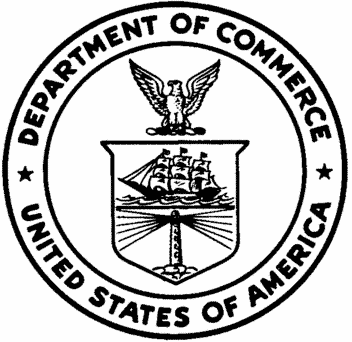
\includegraphics[alt={},width=2cm]{support_files/us_doc_logo.png}\newline % empty curly brackets without alt text is suitable for this logo because it's purely decorative/an "artifact"
  U.S. Department of Commerce\newline
  National Oceanic and Atmospheric Administration\newline
  National Marine Fisheries Service\newline
  Northwest Fisheries Science Center\newline

  \end{minipage}
  \restoregeometry
  \end{titlepage}

\renewcommand*\contentsname{Table of contents}
{
\hypersetup{linkcolor=}
\setcounter{tocdepth}{3}
\tableofcontents
}
\listoffigures
\listoftables

\newpage{}

Please cite this publication as:

Cope, J.M., V. Gertseva, F. Caltabellotta, C. Rosemond, A.D. Whitman.
2025. Status of the Rougheye and Blackspotted Rockfishes stock off the
U.S. West Coast in 2025. NOAA Fisheries Science Center, Seattle, WA.

\newpage{}

\section{Executive Summary}\label{executive-summary}

\subsection{Assessment Model}\label{assessment-model}

\subsection{Reference Points, Stock Status, and
Projections}\label{reference-points-stock-status-and-projections}

\newpage{}

\section{Introduction}\label{introduction}

Testing adding in an introduction for Rougheye and Blackspotted
Rockfishes. There is currently no read of parameters for child
documents.

\subsection{Management History}\label{management-history}

\subsection{Fishery Descriptions}\label{fishery-descriptions}

\subsection{Ecosystem Considerations}\label{ecosystem-considerations}

\newpage{}

\section{Data}\label{data}

\subsection{Stock ID}\label{stock-id}

\subsection{Life History}\label{life-history}

\subsection{Landings}\label{landings}

\subsection{Indices and
Standardization}\label{indices-and-standardization}

\subsection{Composition Data}\label{composition-data}

\subsection{Absolute Abundance}\label{absolute-abundance}

\subsection{Environmental/Ecosystem Indicator
Data}\label{environmentalecosystem-indicator-data}

\newpage{}

\section{Assessment}\label{assessment}

\subsection{Current Modeling Approach}\label{current-modeling-approach}

\subsection{Configuration of the Base
Model}\label{configuration-of-the-base-model}

\newpage{}

\subsection{Modeling Results}\label{modeling-results}

\subsubsection{Parameter Estimates}\label{parameter-estimates}

\subsubsection{Recruitment Estimates and
Deviations}\label{recruitment-estimates-and-deviations}

\subsubsection{Model Fits}\label{model-fits}

\subsubsection{Model Diagnostics}\label{model-diagnostics}

\newpage{}

\subsection{Sensitivity Analyses}\label{sensitivity-analyses}

\newpage{}

\subsection{Management Benchmarks}\label{management-benchmarks}

\newpage{}

\subsection{Projections}\label{projections}

\newpage{}

\section{Discussion}\label{discussion}

\newpage{}

\section{Acknowledgements}\label{sec-acknowledgements}

\newpage{}

\section{References}\label{references}

\newpage{}

\subsection{Tables}\label{tables}

Please refer to the \texttt{satf} package downloaded from
remotes::install\_github(`nmfs-ost/satf') to add premade tables.

\newpage{}

\subsection{Figures}\label{figures}

Please refer to the \texttt{satf} package downloaded from
remotes::install\_github(`nmfs-ost/satf') to add premade figures.

\newpage{}

\section{Notes}\label{notes}

\newpage{}

\section{Appendices}\label{sec-appendix}




\end{document}
